\documentclass[10pt]{article}
\usepackage{fancyhdr, geometry, tikz}
\usepackage{mathpartir}
\usetikzlibrary{positioning}
\pagestyle{fancy}

\lhead{\sf CS 6110 Homework 1}
\rhead{\sf Giang Nguyen (htn26) and Quinn Beightol (qeb2)}

\newcommand{\Rule}[3]{
  [\textsc{#1}]~
  \label{rule:#1}
  \hfill
  \ensuremath{\inferrule{#2}{#3}}
  \hfill
}
\newcommand{\steps}{\longrightarrow}

\begin{document}
\subsection*{\sf 1 Free and Bound Variables}
  % $$
  % % \lambda a. \left (
  % %   \lambda b. \left (
  % %     \lambda c. \left (
  % %      \left( \left ( \left ((a a) (\lambda b. b) \right ) b \right ) c \right ) c
  % %     \right )
  % %   \right )
  % % \right )
  % \left ( (a~a)~(\lambda b. b) \right )
  % $$

  \begin{center} 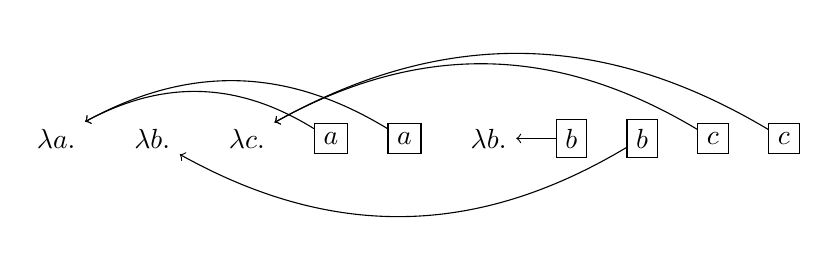
\begin{tikzpicture}[node distance=0.5cm]
    \node (absA) {$\lambda a.$};
    \node (absB1) [right=of absA] {$\lambda b.$};
    \node (absC) [right=of absB1] {$\lambda c.$};
    \node[rectangle, draw] (a1)    [right=of absC] {$a$};
    \node[rectangle, draw] (a2)   [right=of a1] {$a$};
    \node (absB2) [right=of a2] {$\lambda b.$};
    \node[rectangle, draw] (b1) [right=of absB2] {$b$};
    \node[rectangle, draw] (b2) [right= of b1] {$b$};
    \node[rectangle, draw] (c1) [right=of b2]{$c$};
    \node[rectangle, draw] (c2) [right=of c1]{$c$};
    \path[->]
      (a1) edge [bend right]  node {} (absA)
      (a2) edge [bend right]  node {} (absA)
      (b1) edge              node {} (absB2)
      (b2) edge [bend left] node {} (absB1)
      (c1) edge [bend right] node {} (absC)
      (c2) edge [bend right] node {} (absC);
  \end{tikzpicture} \end{center}
\subsection*{\sf 2 Safe Substitution}

$$\left ( \left ( \left (  \left ( \left ( \left ( \right ) \frac{a}{b} \right )  \right ) \right ) \right ) \right ) \big ( \big ) \left ( \frac{a}{b} \right )$$

\subsection*{\sf 3 Small-Step Operational Semantics}
\begin{mathpar}
\Rule{Beta}{}{(\lambda x . e_0)~e_1 \steps e_0 \{ e_1 / x\}}
\Rule{Step Left}{e_1 \steps e'_1}{e_1~e_2 \steps e'_1~e_2}
\Rule{Step Right}{e_2 \steps e'_2}{e_1~e_2 \steps e_1~e'_2} 
\end{mathpar}

\subsection*{\sf 4 $\lambda$-Calculus Encodings}
\subsection*{\sf 5 $\lambda$-Calculus Programming}
\subsection*{\sf 6 Implementing the $\lambda$-Calculus}
\subsection*{\sf 7 Debriefing}
\end{document}
